%
% effekte.tex
%
% (c) 2020 Prof Dr Andreas Müller, Hochschule Rapperswil
%
\section{Numerische Effekte
\label{buch:section:numerische-effekte}}
\rhead{Numerische Effekte}
Die Unzulänglichkeiten der in Computern verwendeten Zahlensysteme haben 
zwei Effekte zur Folge, denen bei der Konzeption eines numerischen
Lösungsverfahrens Rechnung getragen werden muss.

%
% Ausläschung
%
\subsection{Auslöschnung}
{\em Auslöschung} tritt auf, wenn die Differenz zweier ähnlich grosser
Zahlen gebildet wird.
\index{Auslöschung}
Als Beispiel betrachten wir die beiden Zahlen $a=\pi$ und $b=\sqrt{10}$.
Berechnen wir deren Differenz in Octave, erhalten wir:
\verbatiminput{chapters/10-arithmetik/pi10.txt}
Die ersten zwei Stellen von $a$ und $b$ stimmen überein.
Octave zeigt sowohl von $a$ als auch von $b$ 15 signifikante Stellen an.
Ein Vergleich mit einer Berechnung mit noch mehr Stellen zeigt, dass diese
15 Stellen auch zuverlässig sind.
Für die Differenz zeigt Octave ebenfalls 15 Stellen an, doch die
letzte Stelle is falsch, wie zum Beispiel die Berechnung mit 20 Stellen
Genauigkeit zeigt\footnote{Diese Berechnung wurde mit dem
Linux-Kommandozeilenprogramm \texttt{bc} durchgeführt, welches mit
einstellbarer Festkommapräzision von tausenden von Stellen rechnen kann.
Es ist Teil jeder Linux-Distribution.}
\verbatiminput{chapters/10-arithmetik/pi20.txt}
Schreiben wir die Subtraktion in der tabellarischen Form
\begin{center}
\begin{tabular}{>{\tt}r}
 3.16227766016838\\
-3.14159265358979\\
\hline
 0.02068500657859\\
\hline
\end{tabular}
\end{center}
wird erkennbar, dass nur 13 Stellen der Differenz tatsächlich bekannt sind.

Die Rechnung wird in Binärdarstellung etwas klarer.
In der folgenden Tabelle sind die Werte in der mittleren Spalte in
binärer Gleitkommadarstellung gezeigt, Vorzeichen, Exponent und Mantisse
sind zur Verdeutlichung durch ein Leerzeichen getrennt.
Zu Beginn der Mantisse muss man sich eine implizite \texttt{1}
denken, die nicht gespeichert wird.
In der dritten Spalte werden die gleichen Zahlen als binäre Festkommawerten
geschrieben.
Zur Berechnung der Differenz muss der Prozessor die Mantissen ja
zunächst so schieben, dass sie den gleichen Exponenten bekommen,
der Prozessor berechnet also die Differenz implizit in einer
Festkommadarstellung.
\begin{center}
\renewcommand\arraystretch{1.2}
\begin{tabular}{|>{$}c<{$}|>{\tt}r|>{\tt}r|}
\hline 
              & \textrm{Gleikommawert}            &\textrm{Festkommawert}   \\
\hline
\sqrt{10}     & 0 10000000 10010100110001011000010&11.0010100110001011000010\\
\pi           & 0 10000000 10010010000111111011011&11.0010010000111111011011\\
\hline
\sqrt{10}-\pi & 0 01111001 01010010111001110000000& 0.00000{\color{red}10101001011100111}\\
\hline
\end{tabular}
\end{center}
Man kann gut erkennen, dass die Differenz nur 17 signifkante Stellen (rot
hervorgehoben) hat.
Bei der nachfolgenden Darstellung als Gleitkommazahl werden 7 Nullen
hinzugefügt, die aber nichts mit der tatsächlichen Differenz 
$\sqrt{10}-\pi$ zu tun haben.
Aus zwei Zahlenwerten mit einer Genauigkeit von 24 Binärstellen ist ein
Wert mit einer Genauigkeit von nur 17 Binärstellen geworden.
Es sind 7 Binärstellen Genauigkeit ausgelöscht worden.

\begin{beispiel}
\label{buch:beispiel:erfc}
Sei $X$ ein standardnormalverteilte Zufallsvariable, es soll die 
Wahrscheinlichkeit dafür berechnet werden, dass $a\le X\le b$ ist.
In der Wahrscheinlichkeitsrechnung lernt man, dass man dazu die
Verteilungsfunktion
\[
\Phi(x)
=
\frac1{\sqrt{2\pi}} \int_{-\infty}^x e^{-s^2/2} \,ds
=
\frac12 + \frac{1}{\sqrt{2\pi}} \int_0^x e^{-s^2/2} \,ds
\]
der Standardnormalverteilung verwenden kann:
\[
P(a\le X \le b)
= 
\Phi(b) - \Phi(a).
\]
Die Funktion $\Phi(x)$ wird in vielen Bibliotheken nicht direkt zur
Verfügung gestellt, oft ist nur die sogenannte {\em Fehlerfunktion}
\index{Fehlerfunktion}%
\index{$\operatorname{erf}(x)$}%
\[
\operatorname{erf}(x)
=
\frac{2}{\sqrt{\pi}}
\int_0^x e^{-t^2}\,dt
\]
verfügbar.
Die Variablentransformation $t=s/\sqrt{2}$ oder $s=\sqrt{2}t$ macht aus dem
Integral für
$\Phi(x)$ den Ausdruck
\begin{align*}
\Phi(x)
&=
\frac12 + \frac{1}{\sqrt{2\pi}} \int_0^x e^{-s^2/2} \,ds
=
\frac12 + \frac{1}{\sqrt{2\pi}} \int_0^{\sqrt{2}x} e^{-t^2} \,\sqrt{2}\, dt
=
\frac12 + \frac{2}{\pi} \int_0^{\sqrt{2}x} e^{-t^2}\,dt
\\
&= \frac12\biggl(1 + \operatorname{erf}\biggl(\frac{x}{\sqrt{2}}\biggr)\biggr),
\end{align*}
die Fehlerfunktion $\operatorname{erf}(x)$ kann also zur Berechnung der
gesuchten Wahrscheinlichkeit verwendet werden.

In der C-Bibliothek stehen Funktionen zur Berechnung von $\sqrt{2}$ und
$\operatorname{erf}(x)$ für alle zur Verfügung stehenden Datentypen bereit.
Die Tabelle~\ref{buch:table:erfcancellation}
zeigt die Resultate\footnote{Diese Resultate wurden
mit dem Programm \texttt{normal.cpp} Im Verzeichnis
\texttt{buch/chapters/experimente/ausloeschung} von \cite{buch:repo}
berechnet.}
für $a=4.18$ und $b=a+1$.
\begin{table}
\centering
\renewcommand\arraystretch{1.2}
\begin{tabular}{|l|>{$}r<{$}|>{$}r<{$}|}
\hline
Datentyp       & \textrm{Rechnung mit $\operatorname{erf}(x)$}&
\textrm{Rechnung mit $\operatorname{erfc}(x)$}\\
\hline
\texttt{float} & 0.000000\phantom{\mathstrut\cdot10^{-00}}&
6.271826\cdot10^{-17}\\
\texttt{double}& 1.110223\mathstrut\cdot10^{-16}&
6.271826\cdot10^{-17}\\
\texttt{long}  & 6.272110\mathstrut\cdot10^{-17}&
6.271826\cdot10^{-17}\\
\hline
\end{tabular}
\caption{Berechung der Wahrscheinlichkeit $P(4.18\le X\le 5.18)$
einer standardnormalverteilten Zufallsvariable mit Hilfe der
Bibliotheksfunktionen $\operatorname{erf}(x)$ und $\operatorname{erfc}(x)$.
Starke Auslöschung macht die Berechnung mit $\operatorname{erf}(x)$
unbrauchbar.
\label{buch:table:erfcancellation}}
\end{table}

Da die Werte von $\operatorname{erf}(\!\sqrt{2}a)$ und
$\operatorname{erf}(\!\sqrt{2}b)$ fast gleich gross sind, findet 
starke Auslöschung statt.
Beim Datentyp \texttt{float} ist überhaupt kein Unterschied mehr
feststellbar.

Um dieses Problem in den Griff zu bekommen, stellt die C-Bibliothek
zusätzlich die sogenannte {\em komplementäre Fehlerfunktion}
\index{Fehlerfunktion, komplementäre}%
\index{komplementäre Fehlerfunktion}%
\index{$\operatorname{erfc}(x)$}%
\[
\operatorname{erfc}(x) = 1-\operatorname{erf}(x)
\qquad\Rightarrow\qquad
\operatorname{erf}(x) = 1-\operatorname{erfc}(x)
\]
zur Verfügung.
Damit kann die Wahrscheinlichkeit natürlich auch berechnet werden:
\[
P(a\le X \le b)
=
\operatorname{erf}(\!\sqrt{2}b)
-
\operatorname{erf}(\!\sqrt{2}a)
=
(1-\operatorname{erfc}(\!\sqrt{2}b))
-
(1-\operatorname{erfc}(\!\sqrt{2}a))
=
\operatorname{erfc}(\!\sqrt{2}a)
-
\operatorname{erfc}(\!\sqrt{2}b).
\]
Für grosse Werte von $x$ streben die Werte dieser Funktion gegen $0$,
es kann also nicht mehr passieren, dass man einen kleinen Wert zu finden
versucht, indem man zwei vergleichsweise grosse Zahlen voneinander subtrahiert.
In der dritten Spalte von Tabelle~\ref{buch:table:erfcancellation}
sind die Resultate der Berechnung mit Hilfe von $\operatorname{erfc}(x)$
gezeigt.
Der Auschlöschungseffekt ist vollständig verschwunden.
Man kann sogar ablesen, dass die Verwendung des Datentyps \texttt{long double}
dem Problem der Auslöschung ebenfalls nicht begegnen konnte.
Der mit $\operatorname{erf}(x)$ berechnete Wert hat selbst bei Verwendung
dieses längsten verfügbaren Typs nur drei korrekte Dezimalstellen.
\end{beispiel}

%
% Verschmierung
%
\subsection{Verschmierung
\label{buch:subsection:verschiebung}}
Auslöschung kann nicht nur auftreten, wenn zwei fast gleich grosse
Zahlen subtrahiert werden.
Sie kann in etwas weniger offensichtlicher Form stattfinden, wenn
bei der Summation einer Reihe im Vergleich zum Resultat grosse
Zwischenresultate entstehen.
Diesen Verlust an Genauigkeit infolge grosser Zwischenresultate
wird {\em Verschmierung} genannt.
\index{Verschmierung}

\subsubsection{Beispiel: Exponentialreihe $e^x$}
Die Taylor-Reihe
\[
e^x = 1 + x + \frac{x^2}{2!}
+\frac{x^3}{3!}
+\frac{x^4}{4!}
+\frac{x^5}{5!}
+\frac{x^6}{6!}
+\dots
=\sum_{k=0}^\infty \frac{x^k}{k!}
\]
der Exponentialfunktion ist sehr gut geeignet, Werte von $e^x$ für
positive $x$ zu berechnen.
Da der Nenner $k!$ exponentiell schnell anwächst, werden späte
Terme in der Reihe sehr schnell vernachlässigbar klein.

\begin{figure}
\centering
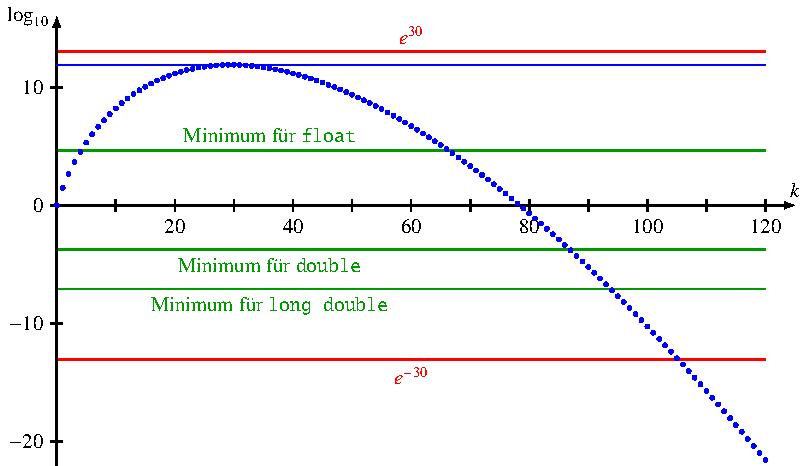
\includegraphics{chapters/10-arithmetik/figures/verschmierung.pdf}
\caption{Verschmierung bei der Berechnung von $e^{-30}$ und $e^{30}$
mit der Exponentialreihe.
Auf der vertikalen Achse ist der Zehnerlogarithmus der verschiedenen
Grössen abgetragen.
Die beiden Werte $e^{30}$ und $e^{-30}$ sind als rote Linien
am oberen und unteren Rand eingetragen.
{\color{blue}Blau} ist der absolute Betrag des Terms $s_k=x^k/k!$ in der
Exponentialreihe.
Die {\color{darkgreen}grünen} Linien zeigen den kleinsten Unterschied,
der zwischen zwei Termen möglich ist, die die Grösse des grössten Summanden
in der Exponentialreihe haben.
\label{buch:figure:expversch}}
\end{figure}
\begin{table}
\centering
\begin{tabular}{|l|>{$}r<{$}|}
\hline
Datentyp            & e^{-30} \\
\hline
\texttt{float}      & -7.2959523438\cdot 10^{\phantom{-}4\phantom{0}}\\
\texttt{double}     &  6.1030424789\cdot 10^{-6\phantom{0}}\\
\texttt{long double}& -1.2489259417\cdot 10^{-8\phantom{0}}\\
\hline
exakt               &  9.3576229688\cdot 10^{-14}\\
\hline
\end{tabular}
\caption{Resultate der Summe der Taylor-Reihe ausgeführt mit verschiedenen
Datentypen zeigt, dass die Genauigkeit der Resultate infolge Verschmierung
vollständig ausgelöscht worden ist.
\label{buch:effekte:taylorsumme}}
\end{table}


Für negative Exponenten erwartet man ein sehr kleines Resultat.
Die Terme der Taylor-Reihe haben alternierende Vorzeichen und werden
zwischenzeitlich sehr gross.
Im Laufe der Rechnung müssen sich also grosse Terme wieder wegheben.
Dies ist in Abbildung~\ref{buch:figure:expversch} illustriert.
Dort sind die Werte $e^{30}$ und $e^{-30}=1/e^{30}$ auf einer logarithmischen
Skala vertikal als {\color{red}rote} Linien eingezeichnet.
Die einzelnen Summanden der Reihe sind in {\color{blue}blau} dargestellt.

\bgroup
\definecolor{darkgreen}{rgb}{0,0.6,0}
Die {\color{darkgreen}grünen} Linien zeigen, welche Genauigkeit mit
verschiedenen Datentypen überhaupt noch möglich ist.
Der \texttt{float}-Typ hat eine Mantisse von 24 bit, eine Zahl $m$ ist
daher nur unterscheidbar von $m(1+\epsilon)$, wenn $\epsilon > 2^{-24}$.
Dies entspricht $24\cdot \log_{10}(2) = 7.22$ Dezimalstellen.
Die {\color{darkgreen}grüne} Linie für den \texttt{float}-Typ ist daher
$7.22$ unter dem Maximum der Terme Exponentialreihe eingetragen.

Beim \texttt{double}-Typen ist die Mantiesse 52 bit lang, beim
\texttt{long double} sind es 63 bit.
Doch selbst beim \texttt{long double} ist die Verschmierung vollständig,
das Resultat für $e^{-30}$ hat nichts mit der Realität zu tun.
Im Gegenteil, sie zeigen eher an, wie gross der verwendete Datentyp ist.
Die {\color{darkgreen}grünen} Linien in Abbildung~\ref{buch:figure:expversch}
befinden sich ungefähr dort, wo die gefundenen Werte
eingetragen werden müssten.
\egroup

In Tabelle~\ref{buch:effekte:taylorsumme} sind die Resultate der
Summierung der Reihe mit verschiedenen Datentypen zusammengestellt.
Alle Summen weichen um mehrere Grössenordnungen vom exakten Wert ab.

\subsubsection{Summationsreihenfolge}
Das Beispiel zur Exponentialfunktion hat gezeigt, wie Verschmierung
die Präzision des Resultates vollständig ausgelöscht hat.
Ein weniger dramatischer Genauigkeitsverlust kann schon bei wenigen
Summanden stark unterschiedlicher Grössenordnung auftreten, wie das
folgende Beispiel aus \cite{buch:kahan-summation} zeigt.

Es soll die Summe $10^4 + \pi + e$ berechnet werden.
Die Rundung kann entweder ganz am Schluss oder nach jeder einzelnen
Addition erfolgen, so wie es der IEEE-754-Standard verlangt.
Es ergibt sich:
\begin{center}
\begin{tabular}{>{$}r<{$}r>{$}r<{$}}
 \textrm{exakte Rechnung}      &\hspace*{2cm}&\textrm{nacheinander} \\[5pt]
10000.0\phantom{0000}&& 10000.0\phantom{0000}\\
+\phantom{0000}3.14159          &&+\phantom{0000}3.14159          \\ \cline{3-3}
                     && 10003.14159          \\
                     && 10003.1\phantom{0000}\\
+\phantom{0000}
    2.71828          &&+\phantom{0000}2.71828          \\\cline{1-1} \cline{3-3}
10005.85987          && 10005.81828          \\
10005.9\phantom{0000}&& 10005.8\phantom{0000}\\
\end{tabular}
\end{center}
Links ist die exakte Addition mit Rundung auf sechs signifikante
Stellen am Schluss durchgeführt, rechts steht die Addition mit Rundung 
nach jeder Operation.
Bereits nach drei Termen zeigt sich ein Unterschied in der letzten Stelle,
der Verschmierung zuzuschreiben ist.

Die unvermeidliche Rundung nach jeder Addition beinträchtigt die Berechnung
jeder unendlichen Summe
\[
s_n
=
\sum_{k=0}^n a_k.
\]
Die naive Berechnung in der Reihenfolge aufsteigender $k$ wird in den
meisten Fällen die Reihenfolge kleiner werdender Terme sein.
Für genügend grosses $k$ werden die zusätzlichen Terme von ähnlicher 
Grössenordnung sein wie die Rundungsfehler, die sich bei den ersten
Termen bereits gebildet haben.

Die Reihenfolge abnehmender $k$ bietet die Chance, dass Rundungsfehler,
die bei der Addition kleiner Terme entstanden sind, bei der Addition
grösserer Terme mit kleinerem $k$ verschwinden im neuen Rundungsfehler
verschwinden.
Dies geschieht allerdings nur, wenn die Beträge der Terme schneller 
wachsen als die Rundungsfehler in den kleinen Termen.
Trotzdem ist es eine gute Idee, eine grosse Summe beginnend bei den
kleinsten Termen zu summieren.

\subsubsection{Kahan-Summationsalgorithmus}
Der Kahan-Summationsalgorithmus versucht, über die sich ansammelnden
\index{Kahan-Summation}
Rundungsfehler in den niederwertigen Stellen in einer separaten 
Variable Buch zu führen.
Um das Prinzip zu verstehen, sei also $s_{n-1}$ eine Teilsumme und $a_n$ der
nächste Term der zur Summe hinzugefügt werden soll. 
Die Summe $s_n=s_{n-1} + a_n$ wird natürlich gerundet.
Die Differenz $c_n = (s_n - s_{n-1}) - a_n$, genau in der Reihenfolge
der Klammern ausgewertet, enthält die durch Rundung verlorenen Stellen.

Der nächste Summand $a_{n+1}$ dürfte kleiner als die Summe $s_{n}$, 
man kann ihn daher um den Betrag $c_n$ korrigieren und damit verlorene
Genauigkeit wiederherstellen.
Wir addieren daher $\bar a_{n+1} = a_{n+1}-c_n$ anstelle von $a_{n+1}$
und erhalten die Summe $s_{n+1} = s_n + \bar{a}_{n+1}$.
Natürlich können wir auch hier wieder den Fehler als
$c_{n+1} = (s_{n+1} - s_{n}) - \bar{a}_{n+1}$ berechnen.
Damit erhalten wir den Algorithmus in
Listing~\ref{buch:list:kahan-algorithmus}.
\lstinputlisting[style=C,float,caption={Kahan-Summations-Algorithmus zur
Vermeidung sich akkumulierender Runungsfehler.},label={buch:listing:kahan-algorithmus}]{chapters/10-arithmetik/kahan.c}
Er verwendet die Funktion \texttt{a(i)}, welche den Term mit Index $i$
der Summe berechnet.
Die Kahan-Summation vervierfacht die Anzahl der Additionen hat aber das
Potential die Akkumulation von Rundungsfehlern fast vollständig zu 
eliminieren.

\begin{beispiel}
Die harmonische Reihe 
\[
h_n
=
\sum_{k=1}^n \frac{1}{k}
\]
kann gegen unten abgeschätzt werden mit Hilfe des Integrals
\[
\sum_{k=1}^n \frac1k
>
\int_1^{n+1} \frac1x\,dx = \log(n+1),
\]
welches divergiert.
Die Folge $h_n$ divergiert also, aber sehr langsam.
Beim numerischen Aufsummieren gibt es ausgiebig Gelegenheit für 
Genauigkeitsverlust.
Am akutesten ist der Verlust, wenn man die Summe mit dem grössten
Term $k=1$ beginnt, eine kleine Verbesserung ist von der umgekehrten
Reihenfolge zu erwarten.

\begin{table}
\centering
\begin{tabular}{|l|>{$}r<{$}|>{$}r<{$}|}
\hline
Methode         &\texttt{float}&\texttt{long double}\\
\hline
vorwärts        &\underline{1}5.403682{\color{gray}70}& 18.99789641385390515 \\
rückwärts       &\underline{18}.807918{\color{gray}55}& 18.99789641385389798 \\
Kahan-Summation &\underline{18.997896}{\color{gray}19}& 18.99789641385389827 \\
\hline
\end{tabular}
\caption{Berechnung der Summe $h_n$ der harmonischen Reihe für $h=10^8$
mit verschiedenen Methoden.
\label{buch:table:kahan}}
\end{table}

Die Resultate der Berechnung von $h_{10^8}$ mit dem \texttt{float}
Datentyp sind in Tabelle~\ref{buch:table:kahan} zusammengestellt.
Die naheliegende Summierung beginnend beim ersten Term führt auf ein
unbrauchbares Resultat.
Beginnt man mit dem kleinsten Term, könnten die Rundungsfehler durch
die späteren grösseren Terme übertönt werden, leider divergiert die
Summe so langsam, dass damit nicht alle Fehler zum Verschwinden 
gebracht werden können.
Es sind nur gerade die Stellen vor dem Komma korrekt.
Die Kahan-Summation vermeidet dieses Problem vollständig.

Zum Vergleich ist in der Spalte rechts in Tabelle~\ref{buch:table:kahan}
die Summe berechnet mit dem Typ \texttt{long double} dargestellt.
Dies zeigt, dass alle signifikanten Stellen der Kahan-Summation korrekt
sind.
\end{beispiel}


